\documentclass[12pt]{report}%␣␣␣␣␣␣autres␣choix␣:␣book,␣report
\usepackage[utf8]{inputenc}%␣␣␣␣␣␣␣␣␣␣␣gestion␣des␣accents␣(source)
\usepackage[T1]{fontenc}%␣␣␣␣␣␣␣␣␣␣␣␣␣␣gestion␣des␣accents␣(PDF)
\usepackage[english]{babel}%english gestion
\usepackage{hyperref}
\usepackage[bottom]{footmisc}
\usepackage[font=small,labelfont=bf]{caption}
\usepackage[newparttoc]{titlesec}
\usepackage[nonumberlist,toc]{glossaries}
\usepackage[export]{adjustbox}
\usepackage[margin=0.95in]{geometry}
\usepackage{setspace} %package pour changer interligne
\usepackage[final]{pdfpages} %import PDF


%All the packages
\usepackage{lmodern,ragged2e,textcomp,lmodern}
\usepackage{graphicx,xcolor,float,fancyhdr}
\usepackage{chngcntr,times,lastpage}
\counterwithout{figure}{chapter}
\usepackage{subcaption,wrapfig,fancyhdr,blindtext}
\usepackage{titletoc,afterpage,transparent}


%Nouvelles commandes
\renewcommand{\familydefault}{\sfdefault} %default font
\newcommand{\periodafter}[1]{#1 -}
\newcommand{\HRule}{\rule{\linewidth}{0.5mm}}
\newcommand{\Mline}{\hrule \mbox{}\\[0.1cm]}
\renewcommand{\thechapter}{\Roman{chapter}}
\newcommand\blankpage{%
    \null
    \thispagestyle{empty}%
    \addtocounter{page}{-1}%
    \newpage}

%FORMAT DU CHAPITRE
\titleclass{\chapter}{straight}
\titleformat{\chapter}[hang]
  {}
  {\normalfont \sffamily \bfseries \large \thechapter. \hspace{0.5cm} }
  {0pt}
  {\normalfont \sffamily \large \bfseries }
\titlespacing*{\chapter}{0pt}{50pt}{18pt}

%FORMAT DE SECTION
\titleclass{\section}{straight}
\titleformat{\section}[hang]
  {}
  {\normalfont \sffamily \bfseries \large \hspace{0.5cm} \thesection \hspace{0.1cm} }
  {0pt}
  {\normalfont \sffamily \bfseries }
\titlespacing*{\chapter}{0pt}{50pt}{18pt}

%FORMAT DE SUBSECTION
\titleclass{\subsection}{straight}
\titleformat{\subsection}[hang]
  {}
  {\normalfont \sffamily \bfseries \large \hspace{1cm} \thesubsection \hspace{0.1cm} }
  {0pt}
  {\normalfont \sffamily \bfseries }
\titlespacing*{\chapter}{0pt}{50pt}{18pt}

%FORMAT DU TEXTE
\onehalfspacing %1.5 interligne
%\usepackage{mathptmx}% http://ctan.org/pkg/mathptmx

\begin{document}

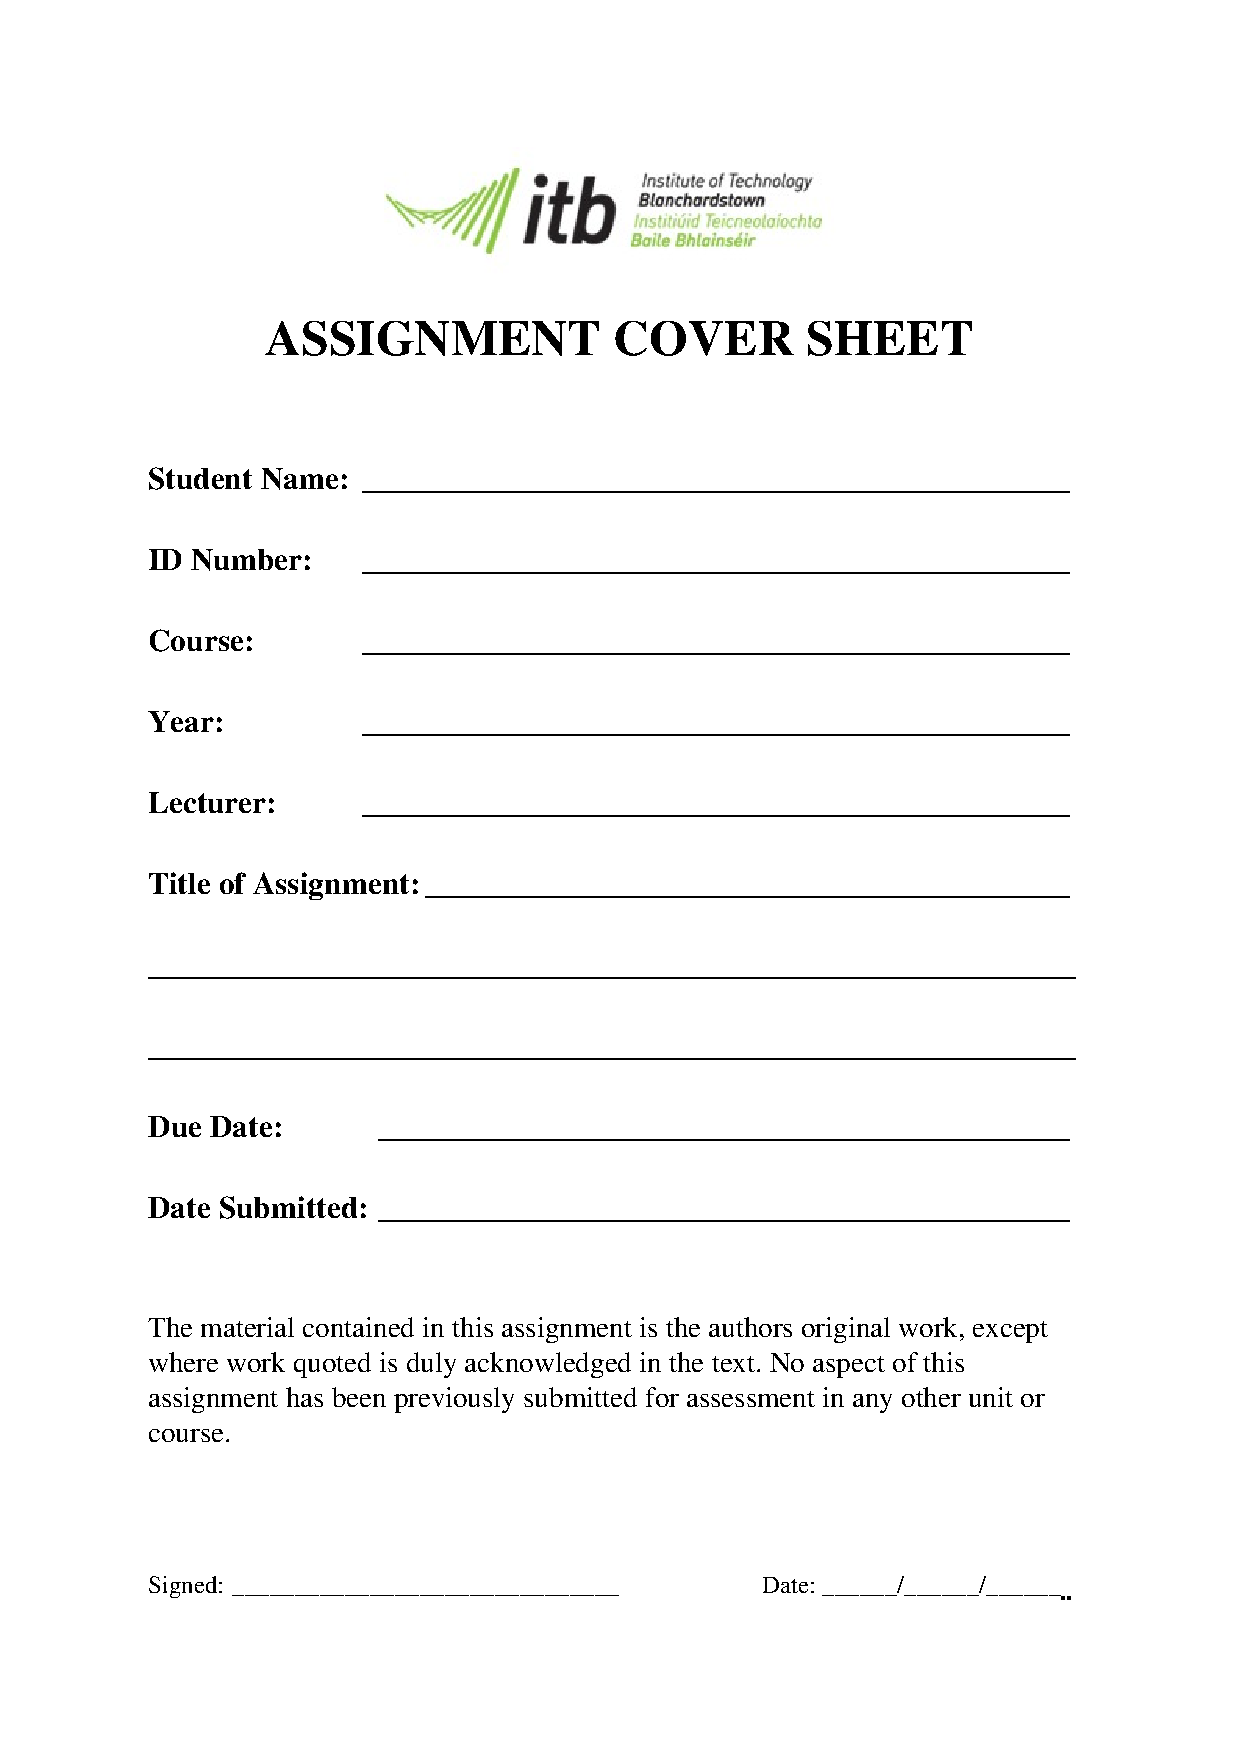
\includepdf[page= 1]{Assign_cover.pdf}

\setcounter{page}{2}

\tableofcontents
\clearpage

\chapter{Abstract}
This report explain the steps in the development of a web application for desktop which is adaptable for other device like smart-phones or tablets, from the conceptual planning and design to the realisation. This application has been realize in group of two, dividing the work according to forces and weaknesses of each. This web site had to be a professional and engaging web application that will enhance the user
experience when using it. 

\chapter{Application}
\section{Technologies}
We used HTML, CSS, JavaScript, jQuery for mobile and JSON to realize the application.\\
For the three main sections, we used one API for each. For the blog, we used Wordpress API's to set up a blog where we are displaying information with the JSON plug-in.\\
For the section called "Pictures", we used Flickr API's to display photos from a Flickr account.\\
For the GoogleMap section, we used the GoogleMap API's.
\section{Design}
\subsection{Form}
The application is composed of an header, a content part and a footer. On the content page you can find four different sections, each one display something different.
\subsection{Background}
For the design, we choose a background pictures related to our subject, houses of champagne in France.\\
\subsection{jQuery Theme}
For the jQuery theme, we used the jQuery theme roller to custom one. We choose colors in relation with nature because we thought this was pretty beautiful and in related to the champagne. Thus, you can find on the application hood and green background and green buttons for example.
\subsection{Pictures}
Pictures are display in grid format. We used CSS code which create the grid in function of the size of each picture because all pictures doesn't have the same original size, thereby the CSS code create the grid taking account of the size and doesn't alter the quality of each pictures keeping the scale of pictures.
\chapter{Group work}
****

\chapter{Research}
****

\chapter{Conclusion}
***

\clearpage
%Breakdown


\end{document}